\documentclass[11pt]{article}
\usepackage[margin=1in]{geometry}
\usepackage{amsmath,amssymb}
\usepackage{listings}
\usepackage{xcolor}
\usepackage{graphicx}
\usepackage{hyperref}

\lstset{
  basicstyle=\ttfamily\footnotesize,
  breaklines=true,
  frame=single,
  language=C++
}

\begin{document}

\noindent\textbf{ECE 759 --- Assignment 4} \hfill Pranav Mehrotra \\

\vspace{1.5em}

\noindent\textbf{GitHub Link:} \url{https://github.com/pmehrotra3/repo759/HW04}

\vspace{1.5em}

\noindent\textbf{Task 1.}\\

\begin{enumerate}
  \item[a)] \texttt{numpy} and \texttt{matplotlib} installed.
  \item[b)] \texttt{nbody.py} was run and the final plot, saved as \texttt{task1.png}, is shown below.
  \begin{center}
    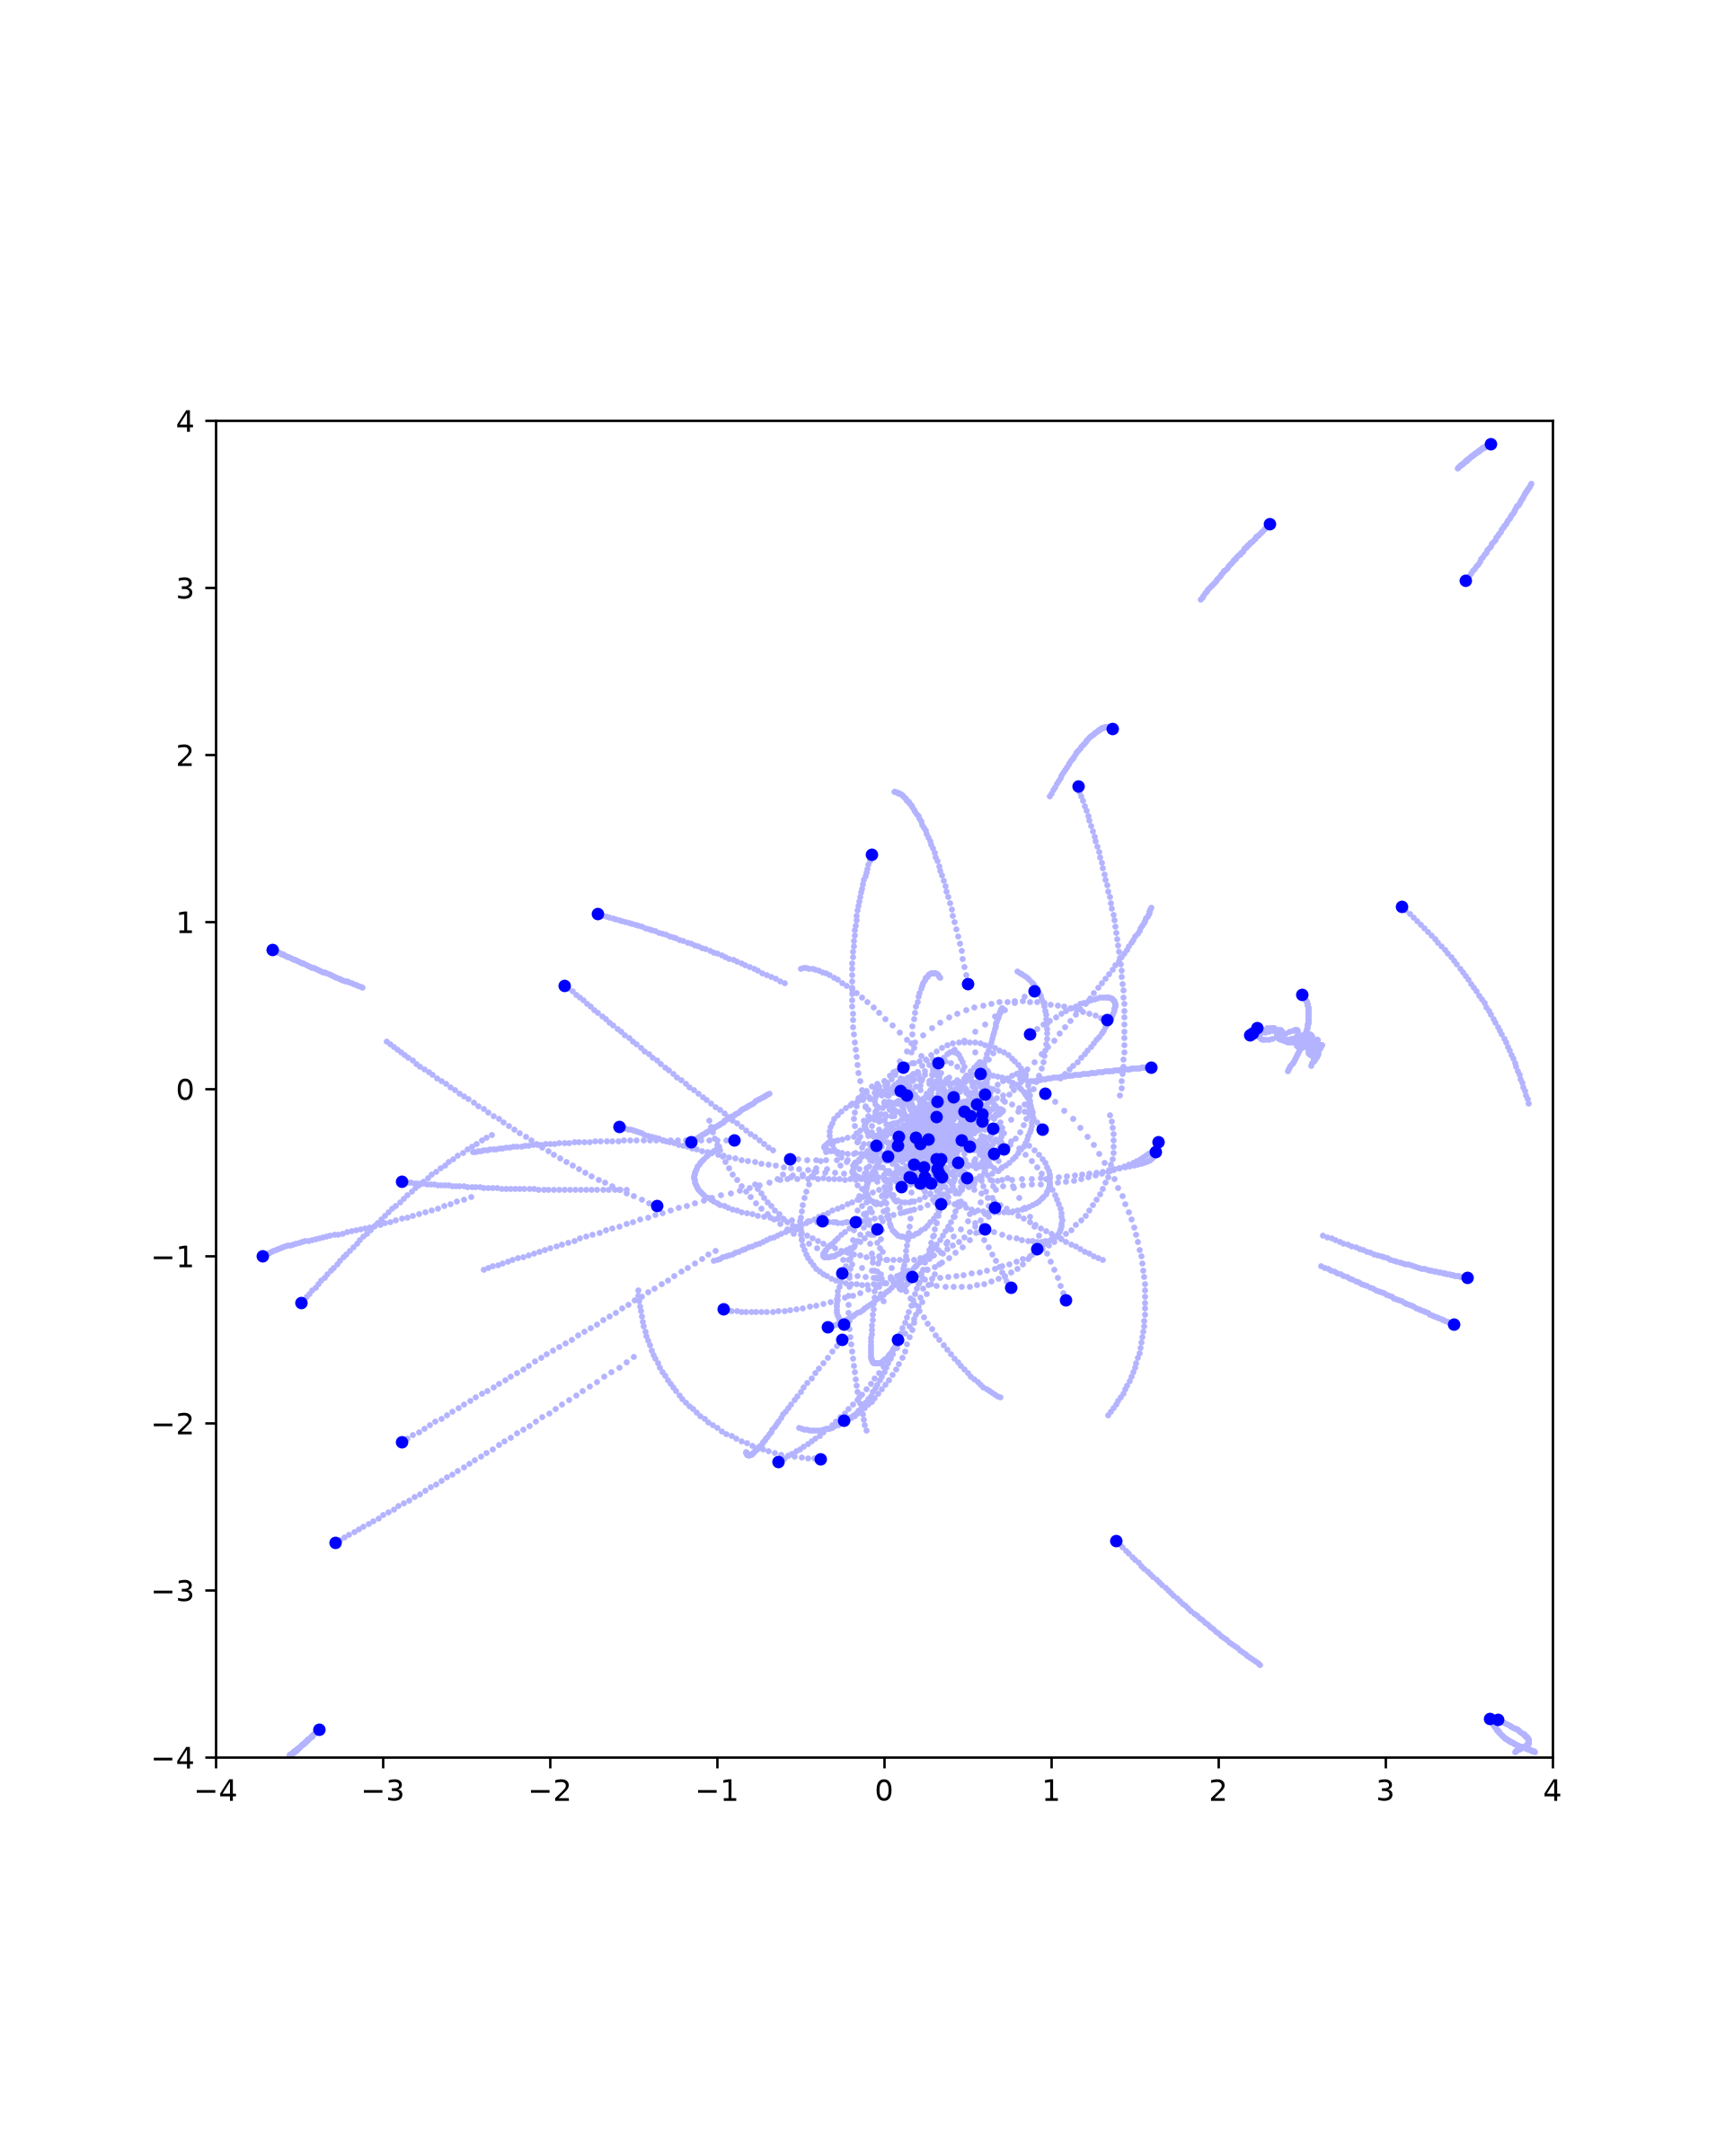
\includegraphics[width=0.6\textwidth]{task1.png}
  \end{center}
\end{enumerate}

\vspace{1.5em}
\noindent\textbf{Task 2.}\\

\begin{enumerate}
  \item[a)] \texttt{task2.cpp} (C++ port of the N-body simulation, completed from the provided skeleton) present in \texttt{HW04} folder.
\end{enumerate}

\newpage
\noindent\textbf{Task 3.}\\

\begin{enumerate}
  \item[a)] \texttt{task3.cpp} (OpenMP version of \texttt{task2.cpp}, taking \texttt{num\_threads} as the third argument) present in \texttt{HW04} folder. \texttt{\#pragma omp parallel for} is used on the outer particle loop of \texttt{getAcc}, the two half-step kicks, the drift and the board-limit check.
\end{enumerate}

\vspace{1.5em}
\noindent\textbf{Task 4.}\\

\begin{enumerate}
  \item[a)] The scheduling policies are implemented in \texttt{task3.cpp}: all parallel loops use \texttt{schedule(runtime)}, and an optional fourth argument (\texttt{static}, \texttt{dynamic} or \texttt{guided}; default \texttt{static}) selects the policy, e.g.\ \texttt{./task3 1000 100 8 dynamic}.
  \item[b)] The plots of the time taken by the N-body simulation versus \texttt{num\_threads} for $N = 1000$ particles and simulation end time $= 100$, one for each scheduling policy (\texttt{task4.pdf}), are shown below.
  \begin{center}
    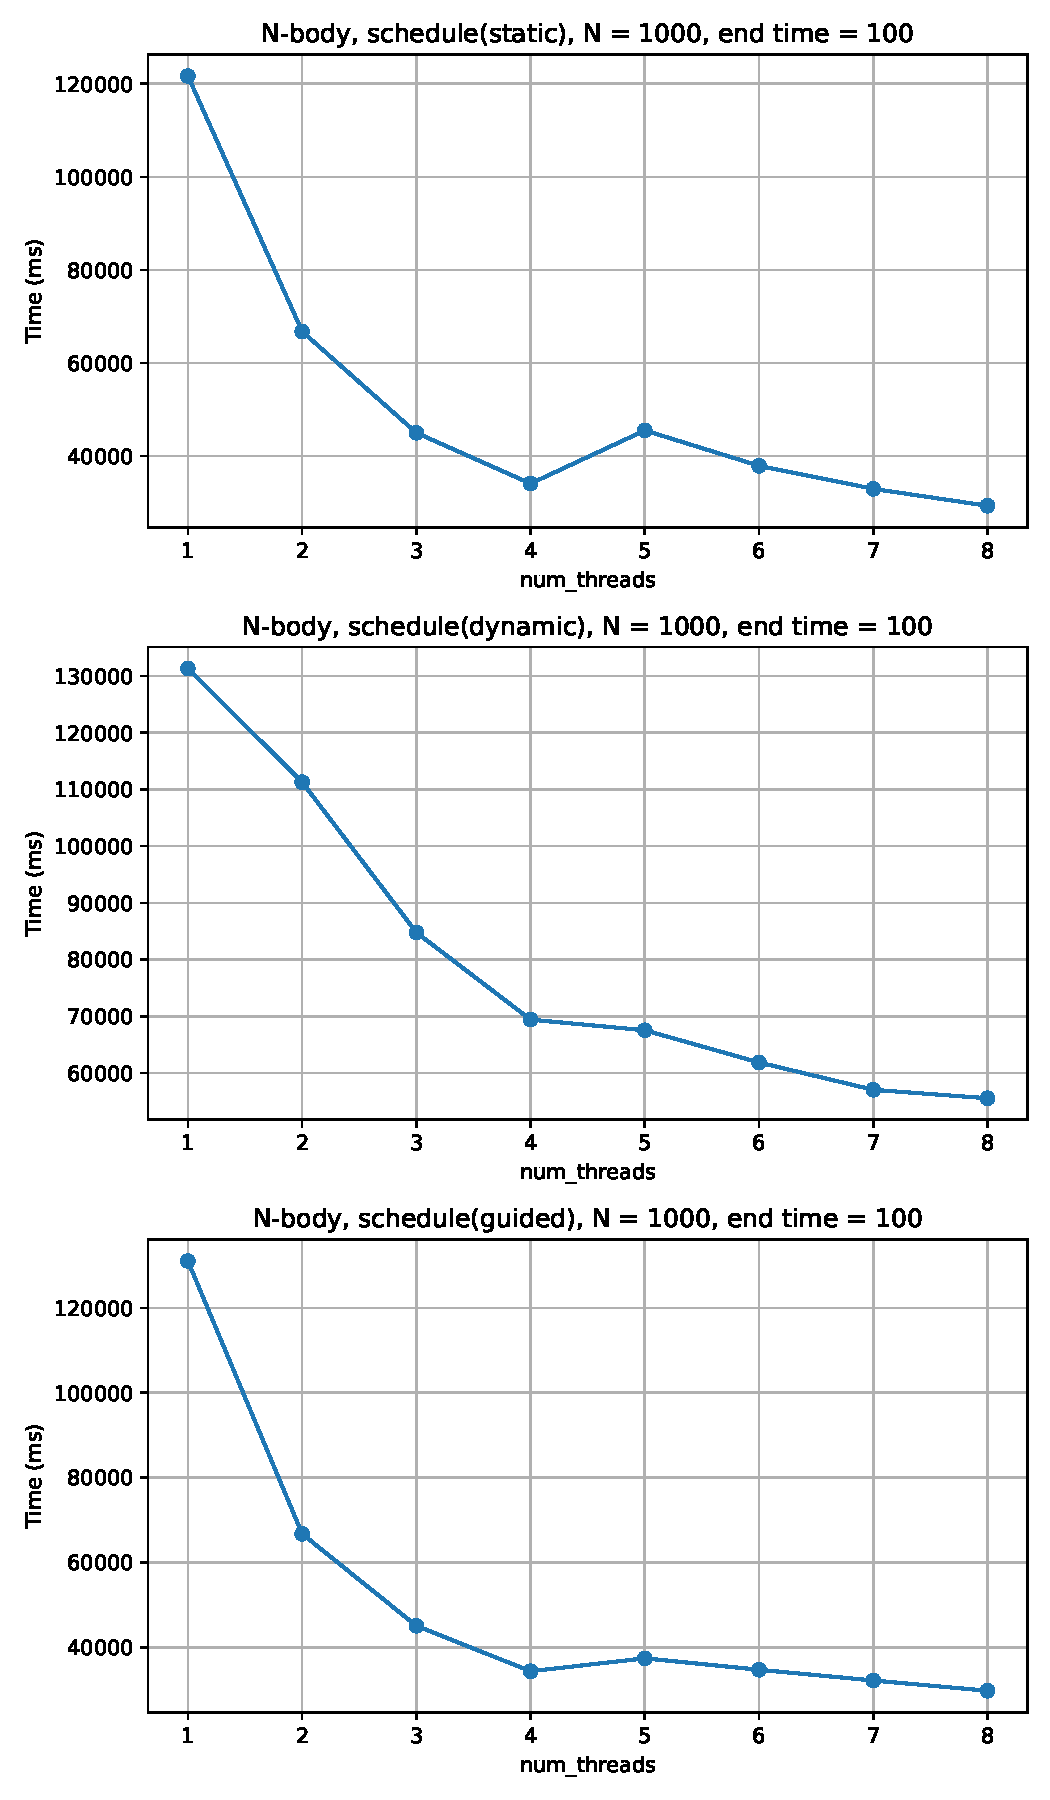
\includegraphics[width=0.42\textwidth]{task4.pdf}
  \end{center}
\end{enumerate}

\end{document}
